% Evaluation
\section{Evaluation}
\label{Evaluation}


We implemented Alano in C++ and evaluated the algorithms in a cluster of 9 servers, each equipped with an Intel Xeon 2.6GHz CPU with 24 hyper-threading cores, 64GB memory and 1T SSD. 
We simulated the network that follows uniform distribution and normal distribution respectively. We consider 500 nodes with radio range 10 in $100\times100$ area following uniform distribution, and more generally, 1000 nodes with radio range 5 following normal distribution $N(50, 15^2)$. The duty cycle is $0.1$, and each time slot represents $20ms$. 
These settings make the network more complicated and realistic than that in \cite{wang2015blinddate, qiu2016talk, sun2014hello, bakht2012searchlight, chen2015heterogeneous, kandhalu2010u, you2011aloha, mcglynn2001birthday, song2014probabilistic, vasudevan2009neighbor}.



We evaluated discovery latency of Alano, Aloha-like~\cite{you2011aloha}, Hello~\cite{sun2014hello}, Hedis~\cite{chen2015heterogeneous}, and Searchlight~\cite{bakht2012searchlight} in partially-connected network. As the deterministic algorithms, Hello, Hedis and Searchlight, only have two states, $\{ON, OFF\}$, we generally assume that when nodes are in $\{ON\}$ state, they transmit and listen with equal probability.
We show that Alano has lower latency, higher discovery rate, and better scalability.

\subsection{Speed: Discovery Latency}

\begin{figure}[!h]
\centering
\subfigure[Uniform Distribution]{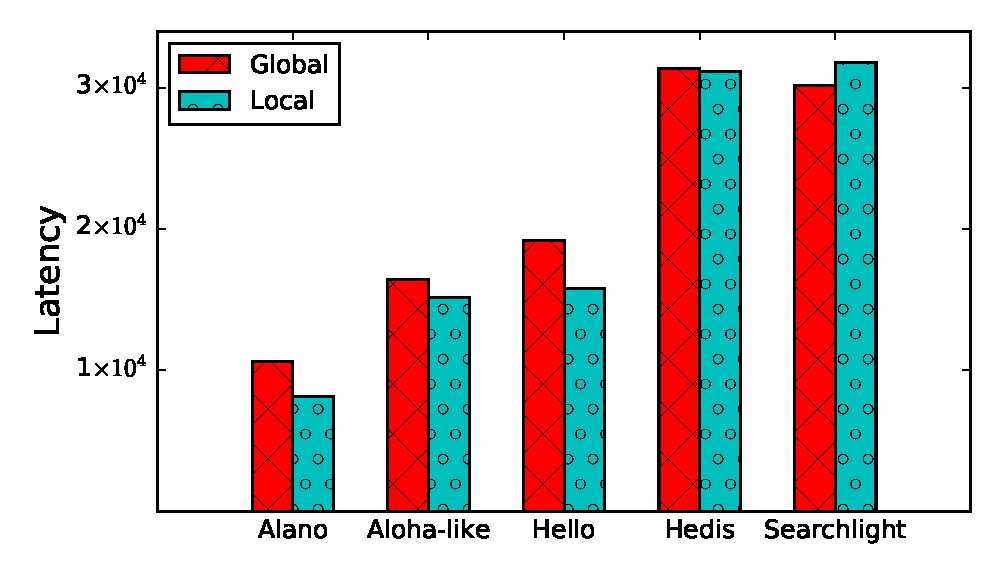
\includegraphics[width=1.65in]{Figure/latency_uniform}}
\hspace{0.01in}
\subfigure[Normal Distribution]{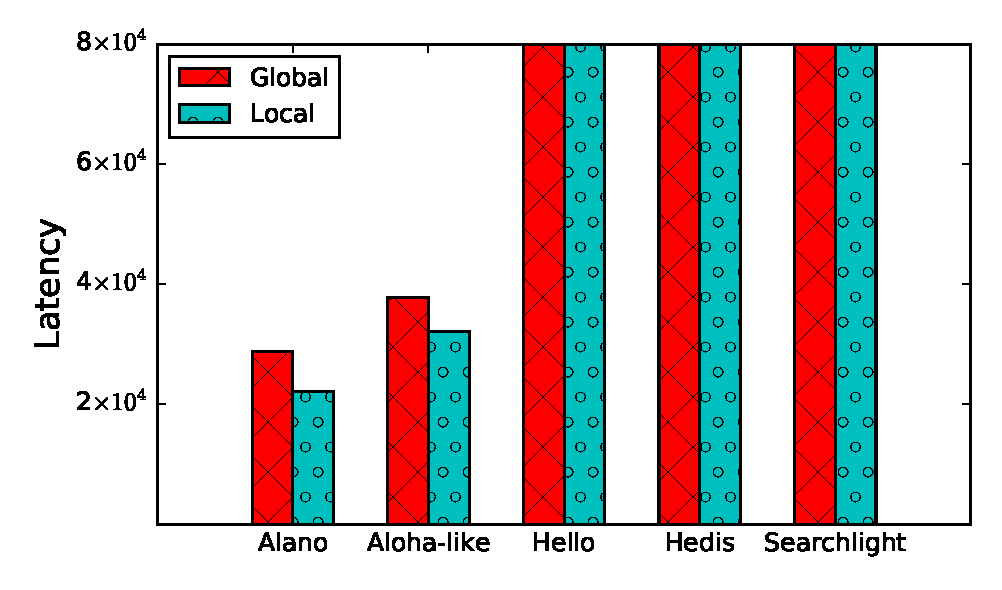
\includegraphics[width=1.65in]{Figure/latency_normal}}
\caption{Alano achieves lower latency.}
\label{fig_latency}
\end{figure}

In Fig. \ref{fig_latency}, when nodes follow uniform distribution, Alano has $53.67\%$ to $5.33$ times lower latency with gloabal duty cycle, and $86.49\%$ to $7.43$ times lower latency with local duty cycle. 
When nodes follow normal distribution, Alano has $31.35\%$ to 24.57 times lower latency with gloabal duty cycle, and $45.94\%$ to $32.32$ times lower latency with local duty cycle. 
The deterministic algorithms Hello, Hedis and Searchlight have high latency, because their design just considered the bounded latency within two nodes. When the network becomes denser and some nodes have more than one neighbors, they cannot discover rapidly, because collisions happen so frequently.


\subsection{Quality: Discovery Rate}

\begin{figure}[!h]

\subfigure[Uniform Distribution with Global Duty Cycle]{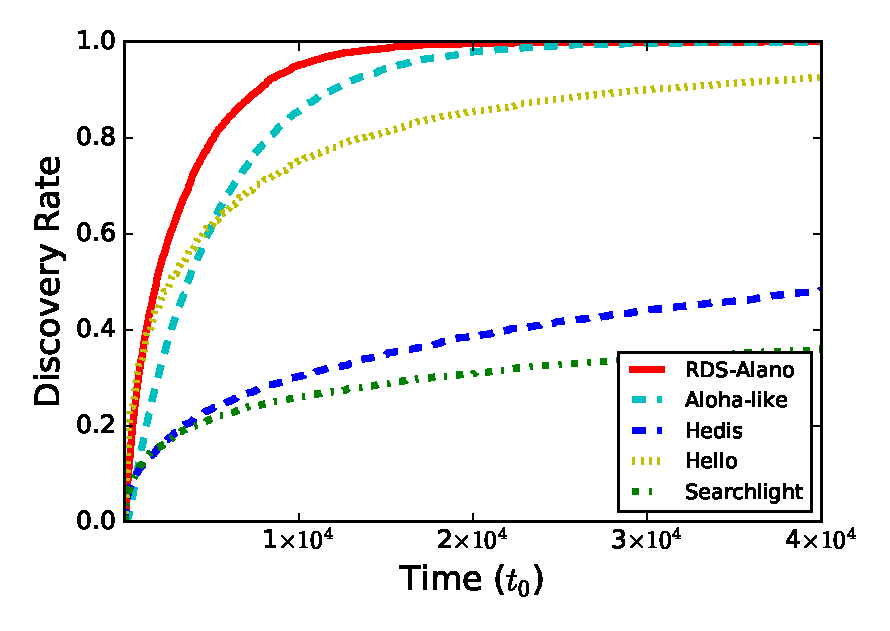
\includegraphics[width=1.65in]{Figure/rate_uniform}}
\hspace{0.01in}
\subfigure[Normal Distribution with Global Duty Cycle]{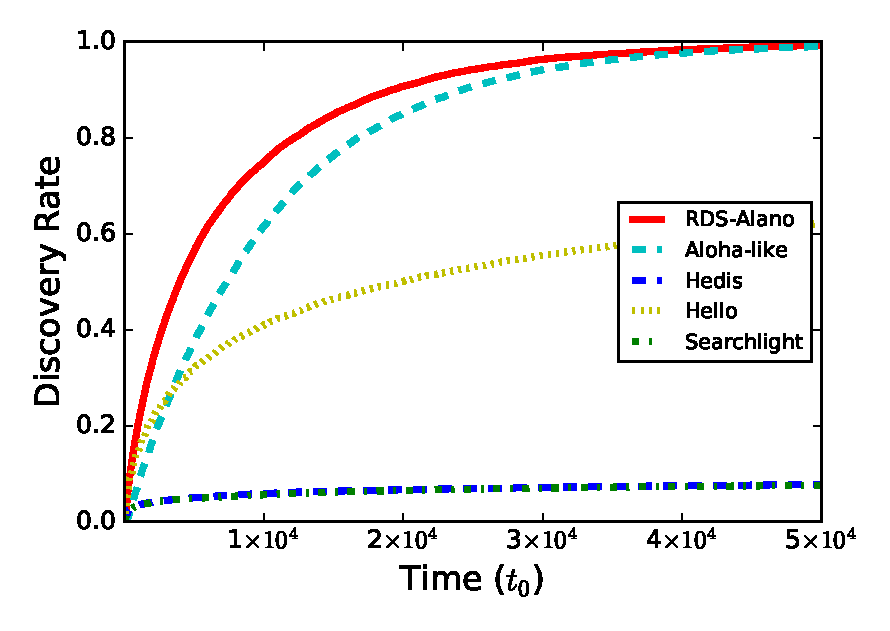
\includegraphics[width=1.65in]{Figure/rate_normal}}
\hspace{0.01in}
\subfigure[Uniform Distribution with Local Duty Cycle]{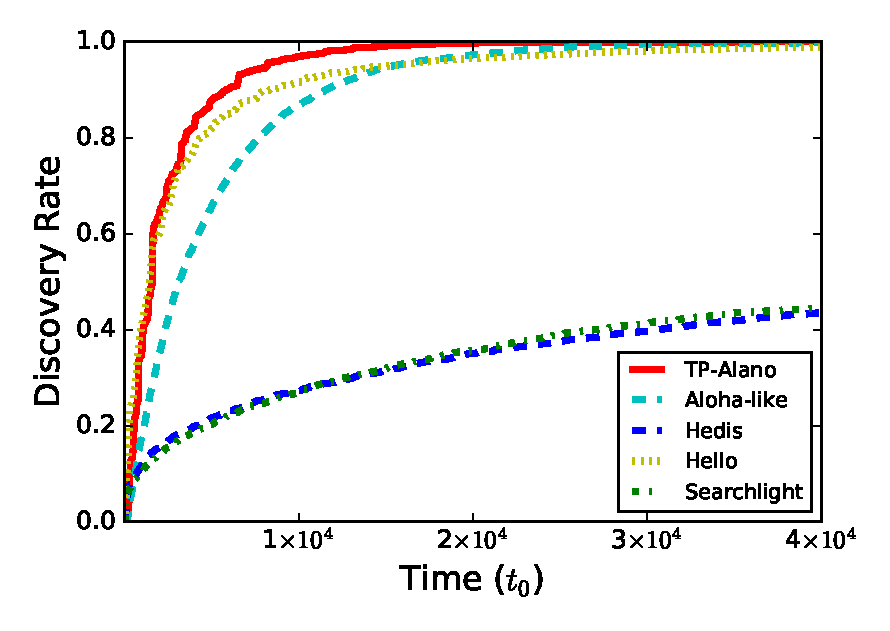
\includegraphics[width=1.65in]{Figure/rate_local_uniform}}
\hspace{0.01in}
\subfigure[Normal Distribution with Local Duty Cycle]{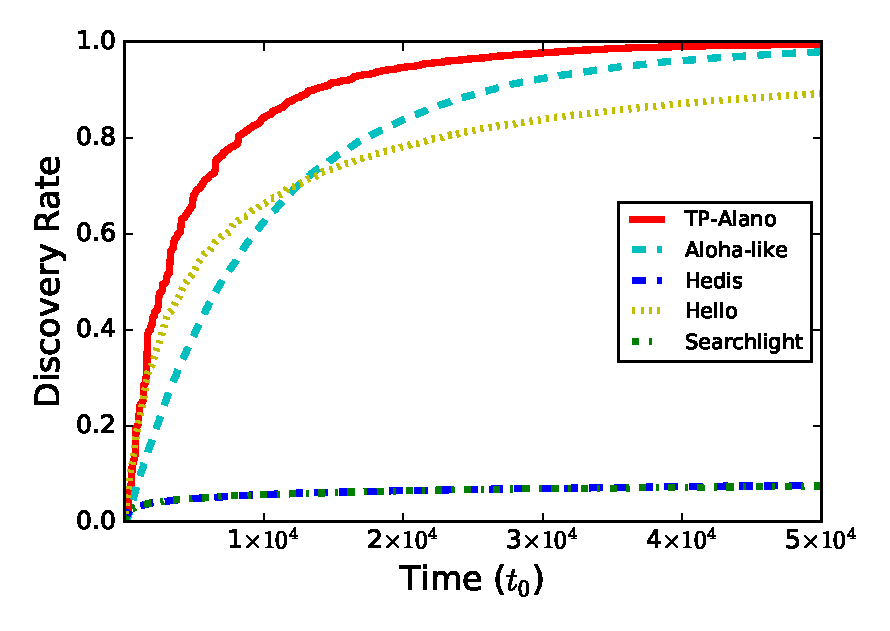
\includegraphics[width=1.65in]{Figure/rate_local_normal}}
\caption{Alano achieves higher discovery rate.}
\label{fig_timerate}
\end{figure}


Fig. \ref{fig_timerate} shows Alano with either global or local duty cycle, has higher discovery rate during the whole course of neighbor discovery in both uniform and normal distribution. The deterministic algorithms Hello, Hedis and Searchlight cannot discover all channels, because of the occurence of collisions. Aloha-like discovers more slowly than Alano when it has discovered a certain number of channels, such as $80\%$ channels in Uniform Distribution with Global Duty Cycle, because it is difficult for pure probabilistic algorithm to deal with the small amount of   undiscovered neighbors.


\begin{figure}[!t]

\subfigure[Uniform Distribution with Global Duty Cycle]{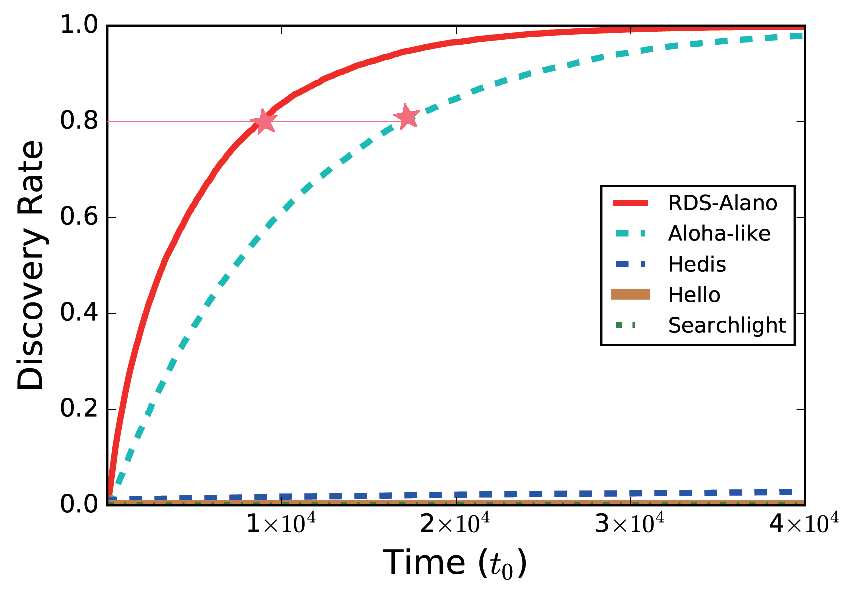
\includegraphics[width=1.65in]{Figure/rate_uniform1}}
\hspace{0.01in}
\subfigure[Normal Distribution with Global Duty Cycle]{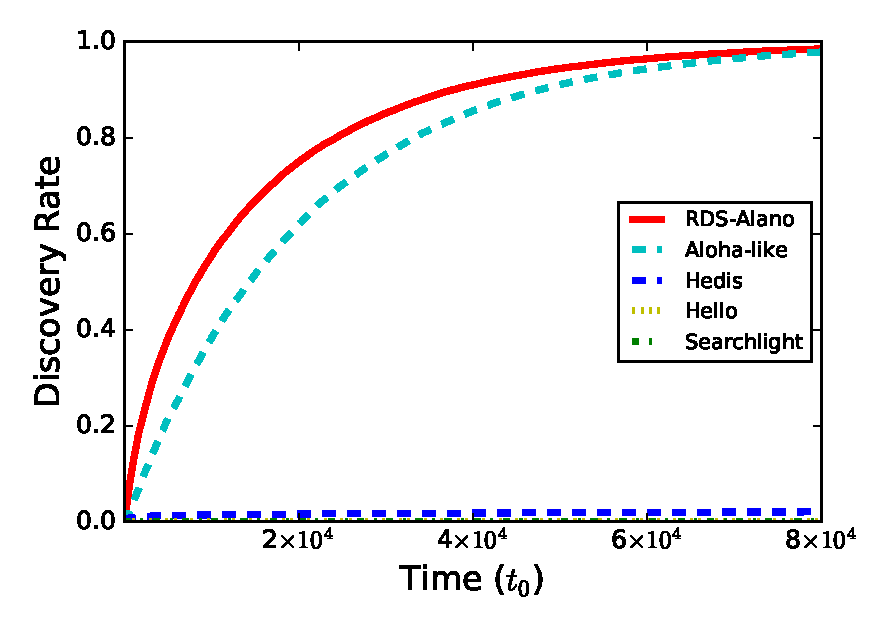
\includegraphics[width=1.65in]{Figure/rate_normal1}}
\hspace{0.01in}
\subfigure[Uniform Distribution with Local Duty Cycle]{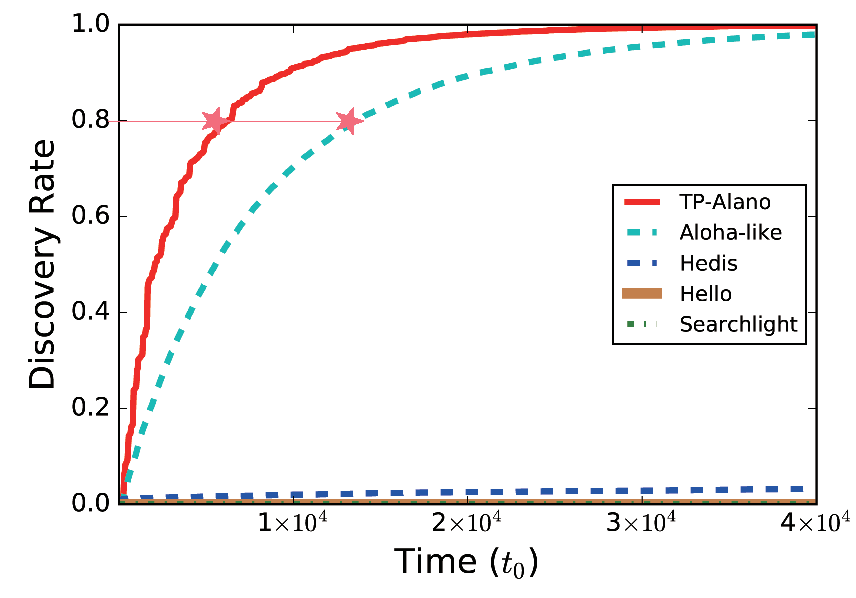
\includegraphics[width=1.65in]{Figure/rate_local_uniform1}}
\hspace{0.01in}
\subfigure[Normal Distribution with Local Duty Cycle]{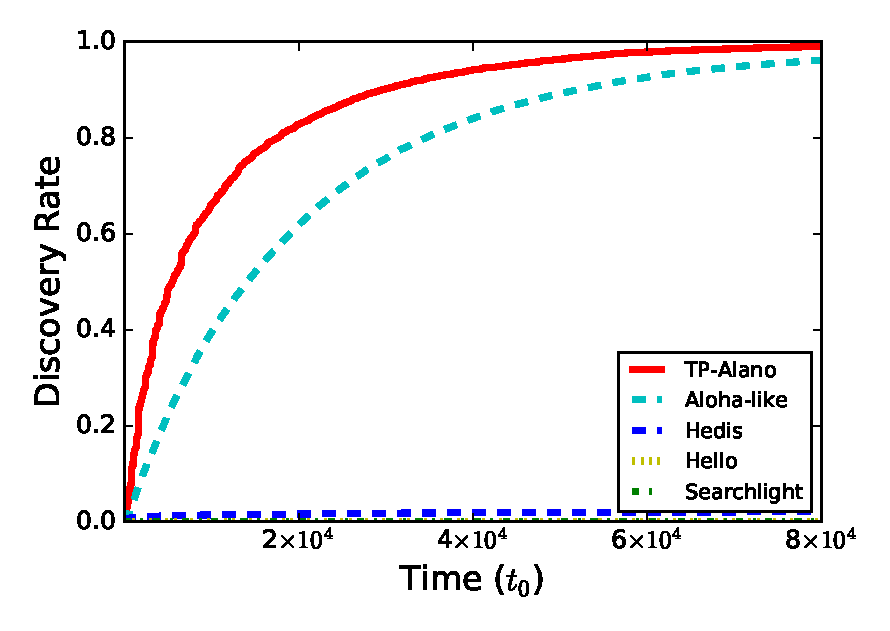
\includegraphics[width=1.65in]{Figure/rate_local_normal1}}
\caption{Alano achieves higher discovery rate in larger networks.}
\label{fig_timerate_large}
\end{figure}

When we increase the number of nodes in the uniform distributed  network from $500$ to $1000$, and the number of nodes in the normal distributed network from $1000$ to $2000$, Fig. \ref{fig_timerate_large} shows that Alano still reaches higher discovery rate all the time with either global or local duty cycle.



\subsection{Scalability: Duty Cycle and Network Density}

\begin{figure}[!h]
\centering
\subfigure[Uniform Distribution]{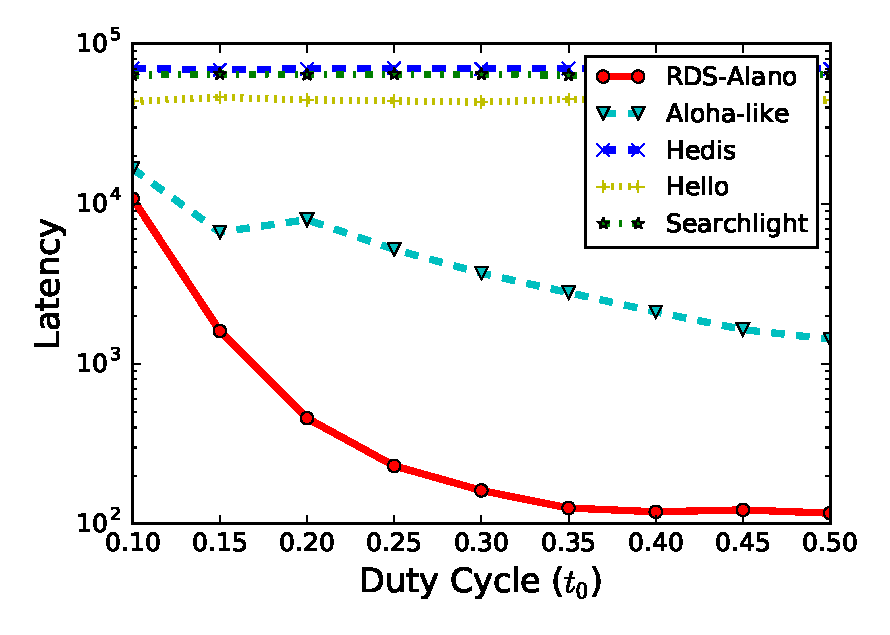
\includegraphics[width=1.65in]{Figure/dutycycle_uniform}}
\hspace{0.01in}
\subfigure[Normal Distribution]{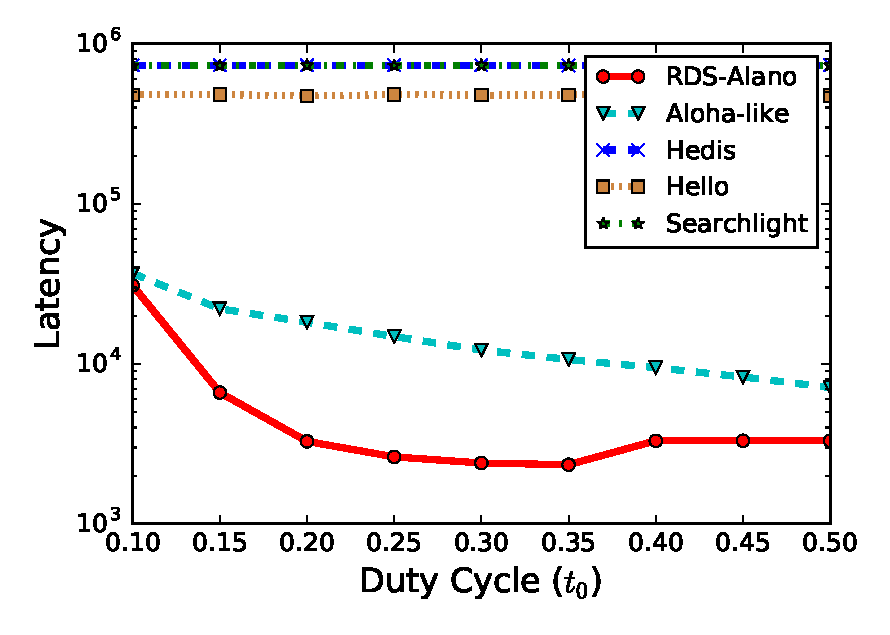
\includegraphics[width=1.65in]{Figure/dutycycle_normal}}
\caption{Alano achieves lower latency in different duty cycle.}
\label{fig_dutycycle}
\end{figure}

\emph{Duty Cycle} 

With different duty cycle, Fig. \ref{fig_dutycycle} shows that Alano has lower latency. Compared with Aloha, Alano has from $53.66\%$ to $11.23$ times lower latency. The latency of Alano and Aloha generally decreases as the duty cycle increases, while Hello, Hedis and Searchlight have high latency due to the collision. In normal distribution, Alano has a small twist with duty cycle $0.35$, because when the duty cycle increases, nodes are more likely to transmit and therefore collide.


\begin{figure}[!h]
\centering
\subfigure[Uniform Distribution]{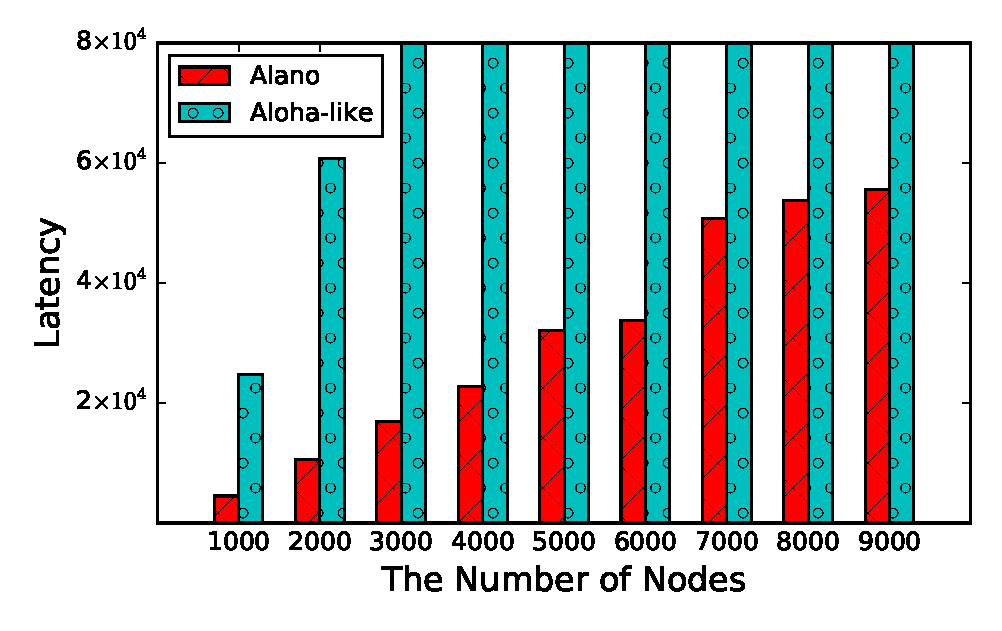
\includegraphics[width=1.65in]{Figure/node_uniform}}
\hspace{0.01in}
\subfigure[Normal Distribution]{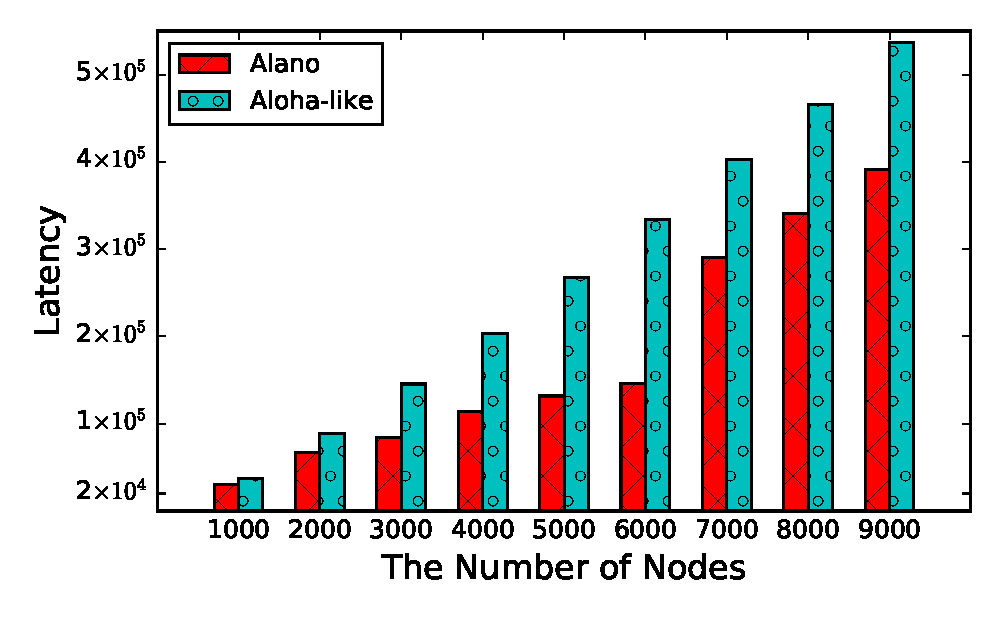
\includegraphics[width=1.65in]{Figure/node_normal}}
\caption{Alano achieves lower latency with different number of nodes.}
\label{fig_node}
\end{figure}

\emph{Network Density} 

When the number of nodes increases and the network becomes denser, Alano still shows $50.16\%$ to $4.52$ times lower latency than Aloha-like in uniform distribution and up to $47.03\%$ in normal distribution in Fig. \ref{fig_node}. Here we compare Alano with Aloha-like, because Hello, Hedis and Searchlight can hardly discover neighbors in denser networks. 


